

\section{Approach}\label{sec:approach}


Our goal is to recover the missing contents in a corrupted video, with consideration of fine details and temporal consistency.
To produce a completed frame $\widetilde{V}_t$ at time $t$, we take total $T$ ($T=5$) frames $\boldsymbol{V}=\msset{V}$, as input to our inpainting network in each data batch. 
The corrupted regions \mdf{in the $T$ frames are indicated by binary masks $\boldsymbol{M}=\msset{M}$} where $M_t(p)=1$ indicates that pixel $p$ is corrupted in frame $V_t$. 
%
 
The detailed architecture of our inpainting network is shown in 
Fig.~\ref{fig:stiNet}.
It consists of three main components. 
The first part is an edge inpainting network (ENet) for structure inference that recovers edges in the missing regions of the input frames.
The second part is a coarse-to-fine texture inpainting network (TexNet) that aims to complete the missing content with visual details under the guidance of hallucinated edges.
The third part leverages the ground truth motion flow as auxiliary constraints to enforce temporal coherence of both the completed edge maps and textures at the training stage.
%The ground truth motion flow is employed to guarantee the consistency of edges and aggregate previously synthesized frames to refine the current frame.
%During the inference stage, only the edge-guided inpainting path is used to complete the target frame, which generates high-quality inpainted results with low time cost.



\subsection{Edge Inpainting Network}
\label{sec:edgenet}
 
The edge inpainting network (ENet) completes image edges in the missing regions to depict scene structures and object shapes.
\mdf{From $T$ neighboring corrupted frames $\boldsymbol{V}$ as well as the corresponding set of binary masks $\boldsymbol{M}$}, a Canny edge detector is first applied to extract the corresponding edge maps $\boldsymbol{E}^{i}$ in the uncorrupted regions. %Notably, the edges in the masked regions in $\boldsymbol{E}^{i}$ are missed. 
%Given the incompleted grayscale images $\boldsymbol{X}^{g}$ of input frame, a canny edge detector is first used to generate initial edge maps. 
The input of ENet is \mdf{the concatenation of} the incomplete grayscale version of $T$ frames $\boldsymbol{V}^{g}$, initial edge maps $\boldsymbol{E}$, and their corresponding masks $\boldsymbol{M}$.
%
As shown in Fig.~\ref{fig:stiNet}, our ENet, denoted by $G^E$, is composed of a two-layer 3D encoder, eight 2D residual blocks, and a two-layer 3D decoder. 
%{\color{blue}Detailed network architecture implementation is listed in Table~\ref{tab:enet-arch1}.}
The 3D encoder and decoder are designed to \mdf{capture temporal coherence which takes large computation consumption. The intermediate 2D residual blocks are efficient in aggregating spatial contexts in large spatial receptive fields. Under a limited number of network parameters, we can adopt more 2D convolution layers thereby obtain larger spatial receptive fields compared to 3D convolutions.
This hybrid 2D and 3D convolution network achieves a good balance between spatial and temporal coherence.}
The inpainted $T$ edge maps 	$\boldsymbol{\widetilde{E}}=\msset{\widetilde{E}}$ are obtained by:
\begin{equation}
	\label{eq:edgenet}
	\boldsymbol{\widetilde{E}}=G^E(\boldsymbol{E},\boldsymbol{V}^{g},\boldsymbol{M}).
\end{equation}

\mdf{Without any auxiliary information, the edge inpainting network ENet can be trained adversarially by}:
%
\begin{equation}
	\label{eq:loss_e_}
	\min\limits_{G^E} \max \limits_{D^E} \big(\mathcal{L}^E_{adv}+\lambda_1 \mathcal{L}^E_{fm}\big),
\end{equation}
%
where the discriminator $D^E$ follows the $70\times 70$ PatchGAN architecture \cite{Isola_2017_CVPR}. 
$\mathcal{L}^E_{adv}$ and $\mathcal{L}^E_{fm}$ are the adversarial loss and feature matching loss respectively. 
$\lambda_1$ is a hyper-parameter to balance the two terms.
%
$\mathcal{L}^E_{adv}$ tends to make the inpainted edge maps follow the distribution of real edge maps by
\begin{equation} \label{eq:edge_adver}
	\begin{aligned} 
		\mathcal{L}^E_{adv}  =&\mathbb{E}_{({E}_t^{gt},{V}_t^{g})}\big[logD^E({E}_t^{gt},{V}_t^{g})\big]\\ 
		+&\mathbb{E}_{({\widetilde{E}_t},{V}_t^{g})}\big[log\big(1-D^E ( {\widetilde{E}_t},{V}_t^{g})\big)\big].
	\end{aligned}
\end{equation}
% 
$\mathcal{L}^E_{fm}$ evaluates the feature-level similarity between ground truth and predicted edge maps, which is defined by:
%Feature matching loss was first proposed in \cite{wang2018high} and has been widely used in recent GANs.
%The feature matching loss is defined as:
\begin{equation}
	\label{eq:edge_fm}
	\mathcal{L}^E_{fm}=\sum_{t=1}^T\sum_{k=1}^L{\frac{1}{N_k}\left\| D^E_k({E}_t^{gt},{V}_t^{g})- D^E_k({\widetilde{E}_t},{V}_t^{g})\right\|_1},
\end{equation}
where $D^E_k$ is the $k$-th layer in the $L$-layer $D^E$, and $N_k$ is the element number of the output of $D^E_k$.
\mdf{We use the feature similarity loss $\mathcal{L}^E_{fm}$ instead of L1 reconstruction loss because that L1 reconstruction loss is sensitive to sparse edges.}
%By considering both feature-level and image-level similarities in Eq.~\eqref{eq:loss_e_}, the edge generator $G^E$ can be trained to produce plausible and structurally rational edge maps.
%Note that the discriminator $D^E$ is not optimized by the feature matching loss term. It plays as a feature extractor to optimize the generator $G^E$ for producing plausible edge maps $\boldsymbol{E}$.
As a result, the proposed hybrid 3D and 2D convolution architecture and the adversarial loss enable our ENet to hallucinate the missing edges accurately and efficiently.
An example of the generated edge map is given in Fig.~\ref{fig:coarse-fine} (a) and (b). 
The stripe pattern on the dog is well inferred from neighboring frames. 


\begin{figure}[t]
	\centering
	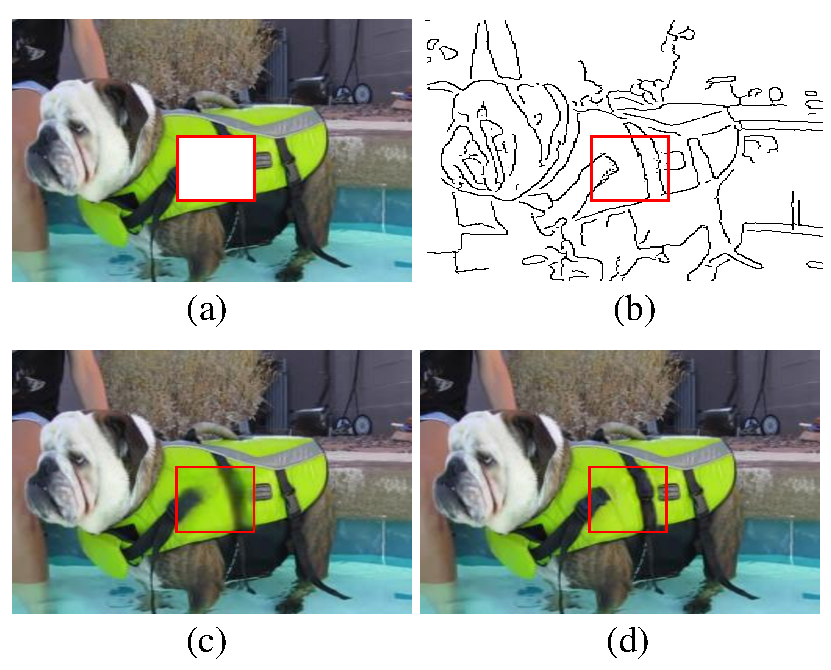
\includegraphics[width=0.8\columnwidth]{coars-fine} 
	\caption{To inpaint missing regions in a corrupted frame (a), our ENet first completes corresponding sparse edges (b), which well represent the structure of the missing contents. Then TexNet progressively replenishes textures under the guidance of synthesized edges from coarse (c) to fine (d).}
	
	\label{fig:coarse-fine}
\end{figure}




\begin{figure}[t]
	\centering
	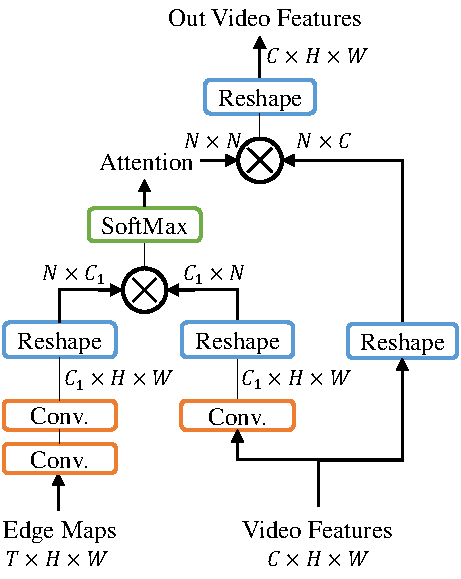
\includegraphics[width=0.65\columnwidth]{SAM}
	\caption{Architecture of the structure attention module. $C$ is number of channels of the input video features, and $N=H\times W$. $\otimes$ represents matrix multiplication. Usually, we set $C_1=C/8$.}
	\label{SEM}
\end{figure} 





\subsection{Edge-Guided Texture Inpainting Network}

 
With the $T$ completed edge maps $\boldsymbol{\widetilde{E}}$ for the $T$ neighboring frames $\boldsymbol{V}$, we then fill the image texture using TexNet.
Notably, the image structure,~\emph{e.g.,} object shapes, is well represented by the completed edge maps $\boldsymbol{\widetilde{E}}$.
Thus, it becomes easier to fill the missing texture with the structural guidance of $\boldsymbol{\widetilde{E}}$.
%
To synthesize realistic frame textures, our TexNet adopts a coarse-to-fine architecture, as shown in Fig.~\ref{fig:stiNet}.
Specifically, TexNet {\color{blue}$G^T$} consists of a coarse inpainting network {\color{blue}$G_c^T$} and a refinement network {\color{blue}$G_r^T$}.
%
%The input of TexNet is the concatenation of  $\boldsymbol{\widetilde{E}}$, $\boldsymbol{V}$, and $\boldsymbol{M}$.
First, the coarse inpainting network consists of a set of 3D convolutions to capture the spatio-temporal contexts from the hallucinated edge maps and the corrupted input frames, and produces a rough completion $\boldsymbol{\widetilde{V}}^i$ for the $T$ frames with colors and textures. {\color{blue}The input of $G^T_c$ is the concatenation of $T$ frames $\boldsymbol{V}$, the synthesized edge maps $\boldsymbol{\widetilde{E}}$, and the masks $\boldsymbol{M}$ to produce $T$ rough inpainting frames in lower resolution:}
{\color{blue}
	\begin{equation}
	\begin{aligned}
	\label{eq:coarsenet}
	\boldsymbol{\widetilde{V}}^i=G_{c}^T(\boldsymbol{V},\boldsymbol{\widetilde{E}},\boldsymbol{M}).
	\end{aligned}
	\end{equation}
}
%The 3D coarse network incorporates neighboring frames by convolutions of the time dimension.
Then, the refinement network takes {\color{blue}the concatenation of} the rough inpainting results $\boldsymbol{\widetilde{V}}^i$, the synthesized edge maps $\boldsymbol{\widetilde{E}}$, and the masks $\boldsymbol{M}$ as inputs to further refine texture details in $\boldsymbol{\widetilde{V}}^i$ with the structural guidance of edges $\boldsymbol{\widetilde{E}}$. 
Notably, only 2D convolutional layers are used in the refinement network to improve inference efficiency. 
%For the corrupted region, our ENet first completes sparse edges which well represent the structure of the missing content, then TexNet progressively replenishes textures under the guidance of synthesized edges.
{\color{blue}
	The refinement network finally reconstructs current frame:
	\begin{equation}
	\label{eq:refinenet}
	\widetilde{V}_t=G_{r}^T(\boldsymbol{\widetilde{V}}^i,\boldsymbol{\widetilde{E}},\boldsymbol{M}).	
	\end{equation}
}
Besides of taking $\boldsymbol{\widetilde{E}}$ as an auxiliary input in the refinement network, we further design a structure attention module (SAM) to fully encode the structural information.
The detailed implementation of SAM is given in Fig.~\ref{SEM}.
\mdf{The input of SAM consists of the intermediate video features extracted from the rough inpainting frames $\boldsymbol{\widetilde{V}}^i$ and the edge maps $\boldsymbol{\widetilde{E}}$.} 
First, the intermediate video features and embedded edge features are interacted to calculate the latent structure-texture correlation via matrix multiplication. 
After a SoftMax operation, the normalized attention map is obtained while it conveys the correlation between sparse structures and video features.
%
The normalized attention map is applied to the intermediate video features, and the structure information is thus embedded in TexNet, which can better extract useful structural information from edges.
{\color{blue}
The main difference between our SAM and self attention module \cite{vaswani2017attention} is that self attention only considers texture correlation, while our SAM focuses on edge-texture correlation to overcome the over-blurry problem in video inpainting.}
By introducing structural guidance in the refinement network, the inpainted content by TexNet becomes more realistic, as Fig.~\ref{fig:coarse-fine} (d) shows.

%The core insight of SAM is to explicitly capture the spatial correlation between edges and textures, which is regarded as a guidance in the texture generation processing.

%Fig.~\ref{fig:coarse-fine} shows an example of our structure-guided inpainting result. 

The coarse inpainting network and the refinement network in TexNet are trained end-to-end in an adversarial manner by:
%
\begin{equation}
	\label{eq:1}
	\min\limits_{G^T} \max \limits_{D^T} \big(\mathcal{L}^{T}_{rec}+\mathcal{L}^T_{adv}\big),
\end{equation}
\mdf{where the discriminator $D^T$ follows the same architecture as $D^E$.}
%
Inspired by \cite{nazeri2019edgeconnect}, the first term $\mathcal{L}^{T}_{rec}$ is the $l_1$-reconstruction loss to measure the difference between predicted video frames and the ground truth video frames $\boldsymbol{V}^{gt}$.
Differently, we penalize both \mdf{the single refined frame $\widetilde{V}_t$ and the coarse predictions of $T$ frames $\boldsymbol{\widetilde{V}}^i$} by:
\begin{equation}
		\label{eq:loss_rec}
	\begin{aligned}
		\mathcal{L}^{T}_{rec}&=\frac{1}{\left\|M_t \right\|_1}\left\|(\widetilde{V}_t-V^{gt}_t)\odot M_t\right\|_1,\\ 
		&+\lambda_2*\frac{1}{\left\|\boldsymbol{M} \right\|_1}\left\|(\boldsymbol{\widetilde{V}}^i-\boldsymbol{V}^{gt})\odot \boldsymbol{M}\right\|_1,
	\end{aligned}
\end{equation}
where $V^{gt}_t$ denotes the ground truth frame of time $t$, and $M_t$ is the corresponding binary mask. 
%
The extra adversarial loss $\mathcal{L}^T_{adv}$ is introduced in Eq.~\eqref{eq:1} to promote the visual realism of the generated frame $\widetilde{V}_t$ by:
	%$\mathcal{L}^I_{adv}$ is defined as:
	\begin{equation}
		\label{eq:inp_adver}
		\mathcal{L}^T_{adv}=\mathbb{E}[logD^T(V^{gt}_t)]+\mathbb{E}[log\big(1-D^T(\widetilde{V}_t)\big)].
	\end{equation}
%$\mathcal{L}^T_{adv}$ enforces the generated frame to be more realistic.


The coarse and refinement networks can be effectively trained jointly with the combined loss of $\mathcal{L}^T_{rec}$ and $\mathcal{L}^T_{adv}$.
The results in Fig.~\ref{fig:coarse-fine} (c) and (d) show that the coarse network completes the missing content with rough textures under the structure guidance of inpainted edges and the refinement network exactly refines the inpainting results with more sharp contours and realistic textures.

% enables the TexNet to first give a coarse inpainting results, and then refine the results with the structure guidance.
%It can be seen that the coarse-to-fine architecture


 

\subsection{Flow-Guided Temporal Coherence Enhancement}
\label{sec:fec}
Besides the structural guidance, motion information is also considered in our method to enhance temporal consistency among the recovered frames.
We employ optical flows in the training stage of both ENet and TexNet \mdf{using self-supervision of neighboring frames.}
A set of flow maps \(\boldsymbol{O}\) between the current frame $V_t^{gt}$ and its neighboring frames are generated using a pre-trained flow extraction network, such as FlowNet2.0~\cite{Flownet_2017_CVPR}.
Specifically, \(\boldsymbol{O}\) consists of four flow maps \((O_{t\Rightarrow t-7}, O_{t\Rightarrow t-3}, O_{t\Rightarrow t+3}, O_{t\Rightarrow t+7})\).
 
 
In terms of the ENet which completes the missing edges, \(\boldsymbol{O}\) is used to first warp the neighboring edge maps to the current frame, and then compute the consistency between neighboring edge maps.  
A flow-guided edge consistency loss is defined as:
%
\begin{equation}
	\label{eq:flow_edge}
	\mathcal{L}^E_{flow}=\sum_{k}\frac{1}{\left\|M_{t} \right\|_1}\left\|\Big(\widetilde{E}_{t}-\phi\big(O_{t\Rightarrow t+k},E_{t+k}^{gt}\big)\Big)\odot M_{t}\right\|_1,
\end{equation}
where $\phi\big(O_{t\Rightarrow t+k},E_{t+k}^{gt}\big)$ is the warping operation which warps a neighboring edge map $E_{t+k}^{gt}$ to the target frame according to the estimated optical flow $O_{t\Rightarrow t+k}$.
$k$ denotes the index of neighboring frames ($k\in \left\{-7,-3,+3,+7 \right\}$). 
\mdf{By introducing this additional flow-guided edge consistency loss $\mathcal{L}^E_{flow}$ when training ENet, the original loss function (Eq.~\eqref{eq:loss_e_}) becomes:}
\begin{equation}
\label{eq:loss_e}
\min\limits_{G^E} \max \limits_{D^E} \big(\mathcal{L}^E_{adv}+\lambda_1 * \mathcal{L}^E_{fm}+\mathcal{L}^E_{flow}\big).
\end{equation}

 

\mdf{Similarly, when we train the TexNet, we further enforce the temporal coherence of synthesized neighboring frames via a flow-guided texture consistency $\mathcal{L}^T_{ftc}$ by:} 
\begin{equation}
	\label{eq:inp_flow}
		\mathcal{L}^T_{flow}=\sum_{k}\frac{1}{\left\|M_{t} \right\|_1}\left\|\Big(\widetilde{V}_{t}-\phi\big(O_{t\Rightarrow t+k},V_{t+k}^{gt}\big)\Big)\odot M_{t}\right\|_1,
	\end{equation}
where $k \in \{-7,-3, 3, 7\}$, and $\phi\big(O_{t\Rightarrow t+k},V_{t+k}^{gt}\big)$ warps the neighboring frame $V_{t+k}^{gt}$ to the target frame using the estimated flow $O_{t\Rightarrow t+k}$. 
\mdf{The flow warping loss $\mathcal{L}^T_{flow}$ is added to the objective function of TexNet, which converts Eq.~\eqref{eq:1}
to:}
\begin{equation}
\label{eq:1_}
\min\limits_{G^T} \max \limits_{D^T} \big(\mathcal{L}^{T}_{rec}+\mathcal{L}^T_{adv} +\mathcal{L}^T_{flow}\big).
\end{equation}

After adding the motion guidance to both the training processes of ENet and TexNet, the temporal consistency can be enhanced in both edge generation and texture inpainting.
Since the motion is only used in the training stage, the inference of the proposed structure-guided inpainting method is efficient and effective.
 






	